\section{The DL\_POLY Java Graphical User Interface}
\index{Java GUI}\label{javagui} The DL\_POLY Java GUI II is an upgrade of the
original (Mark I) version of the GUI and incorporates several new features.
First among these is the Graphical Molecular Editor, which allows the user to
build complex organic structures and replicate them to create systems for
simulation with DL\_POLY. To accomplish this the GUI has two graphical modes:

\begin{itemize}
\item View - for simply viewing the molecular structure in a DL\_POLY CONFIG
  file and also carrying out certain global operations (i.e. affecting the
  whole configuration) such as insertion of water molecules, replication etc.
  Which do not change the contents of the CONFIG file as such, but augment
  them in some way. This mode is equivalent to the previous, sole mode of
  operation of the Mark I version of the GUI.  
\item Edit - for graphically editing the structure of a configuration,
  changing the identities of molecules or atoms, adding or deleting molecules,
  parts of molecules or atoms.
\end{itemize}
Secondly, improvements have been made to the force field builders, which now
include several new Java classes related to system structures and molecular
entities. This will hopefully allow incorporation of additional force fields
more easily than before.

The GUI retains the advantages inherent in the previous version, particularly
in the free availability of Java, a product of Sun Microsystems, and its
portability to all computers that support the Java language. We continue to
supply the code as source (though the executable is also included) so it may
be developed as desired by users with special needs, provided they are of
course willing to learn the Java language.

Other aspects of the new GUI the user should be aware of are as follows:

\begin{enumerate}
\item {\bf The \DD{} Java GUI is not an applet. It is a full Java
application program and cannot be run from within an internet
browser.}
\item {\bf The appearance of the GUI, its windows and browsers
etc may vary from system to system. The broad appearance will remain
the same as will the functionality. This is merely an aspect of Java
portability.}
\item {\bf \label{atomnames}
For the purpose of rendering different atom types in a
configuration, the GUI requires the adoption of a naming convention
based on the Periodic Table. Up to eight characters may specify an
atom name, but the first two must be taken from the proper chemical
symbol. If the chemical symbol is a single letter, the underscore (\_)
must be used. Thus hydrogen and oxygen have the names O\_ and H\_,
while copper and sodium have Cu and Na respectively. Failure to
follow this convention results in the `grey ball' syndrome. The only
exceptions to these rules are the use of symbols OW and HW for oxygen
and hydrogen in water molecules. Other atom naming conventions can be
fitted into this scheme by extension beyond two characters. The GUI
exploits this in the Dreiding\index{force field!Dreiding}
\cite{mayo-90a}, OPLS\index{force field!OPLS} \cite{jorgensen-84a}
and Ceramics\index{force field!Ceramics} \cite{lewis-85a,bush-94a} 
force fields. The user may see what the atom
names are in these force fields by inspecting the MINDREI, MINIOPLS and
CERAMICS files in the java subdirectory, or by listing them from the
Information menu of the GUI (see section \ref{infomenu}).}
\end{enumerate}

\section{Compiling the Java GUI}

The first requirement for compiling the Java GUI is the availability of the
Java software. For national supercomputers and the like, Java should already
be available. To install Java on local machines, the Java home page at the Sun
Microsystems website http://java.sun.com provides the Java Development Kit
(JDK 1.4 or above) for any particular computer. Installation instructions are
available from the same site, and are generally straightforward. Once the JDK
is installed, the DL\_POLY Java GUI may be compiled.

The source code for the Java GUI is found in the DL\_POLY java subdirectory.
On entering this type the command:

\vspace{0.25cm}
{\em javac *.java}
\vspace{0.25cm}

\noindent
which will compile the java source code and construct the Java classes
(i.e. the Java executable ‘objects’). Next it is necessary to make a Java
‘jar’ file from the classes. This neatly encapsulates, in a single file, all
of the GUI Java classes. (The jar file effectively becomes the GUI 
executable, which in fact is transportable between
systems.) This is done with the command:

\vspace{0.25cm}
{\em jar -cfm GUI.jar manifesto *.class About\_DL\_POLY Acknowledge
CERAMICS MINIDREI  MINIOPLS WATER.300K TestInfo Licence Disclaimer}
\vspace{0.25cm}

\noindent
the jar command thus works somewhat like the UNIX tar command. Note
particularly the requirement to incorporate the file ``manifesto'', which is
one of the files in the java subdirectory. The contents of this file inform
the java program which of the incorporated classes represents the entry point
at execution. (It follows that this file should never be deleted!) The files
listed after the *.class inclusion are information the GUI requires to operate
properly. Note that both the javac and jar commands have been combined in the
unix script `build’, which you will find in the java directory.  Invoke this
by typing the command

\vspace{0.25cm}
{\em ./build}
\vspace{0.25cm}

\noindent
The result of this command is the GUI.jar file, which becomes the working
GUI. In addition to compiling the Java source, it is necessary to compile some
FORTRAN programs that the GUI calls upon to perform some of the
calculations. Inside the java subdirectory are the lower directories GDF and
SKW. These contain programs for calculating van Hove correlation functions and
dynamic structure factors respectively. Enter each of these directories and
type `make’ to build the FORTRAN
programs. This will complete the build of the GUI. Note it may be necessary to
change a few of the parameters in the makefiles for these, such as the
specification of the FORTRAN77 compiler or the C compiler.

\section{Starting the Java GUI}

The GUI.jar file is universally transportable. Once created it can be shipped
to any system where Java is featured and it will run just the same (though the
various windows may look a little different). In the case of MS Windows
machines, it can be activated by double-clicking on the file icon. It is
normal practice to run the GUI from within the DL\_POLY execute subdirectory,
which makes it easy to locate the files it needs from within the DL\_POLY
directory structure. (Users who experience strange problems running the GUI
may find that reverting to this practice resolves the problems.) Assuming you
are in the execute directory, to start the GUI in a linux or MS Windows
command window type the command:

\vspace{0.25cm}
{\em java -jar ../java/GUI.jar}
\vspace{0.25cm}

\noindent
Unix users may alternatively use the gui script in the execute subdirectory,
which incorporates the syntax of this command. After a minute or two, the GUI
Graphics Window and the Monitor Window (figure 1) will open onscreen. Both of
these windows may be handled in the usual X manner, e.g. moved with the mouse,
by clicking and dragging the header panel. The size of each may be changed by
clicking and dragging from a corner or edge. The usual window widgets for
hiding, enlarging or closing are present. However note that the close widget
has been disabled for the Monitor Window. The GUI opens in the View mode.

~

\vskip 5mm
\centerline{\psfig{figure=javagui.ps,height=11.5cm}}
\centerline{Figure 1: The Java GUI and Monitor window}
\vskip 5mm

~

\noindent
Both of these windows may be handled in the usual X manner, e.g. moved
with the mouse, by clicking and dragging the header panel. The size of
each may be changed by clicking and dragging from a corner or
edge. The usual window widgets for hiding, enlarging or closing are
present. However {\bf note that the close widget has been disabled for
all Java GUI windows except the Graphics Window}.

If the colour scheme of the GUI offends, try the command:

\vspace{0.25cm}
{\em java -jar ../java/GUI.jar scheme}
\vspace{0.25cm}

\noindent where {\em scheme} is one of the following: {\bf photo,
monet, picasso, vangogh, cezanne} or {\bf mondrian}, 
any of which may be more pleasing. The default colour scheme 
is {\bf picasso}.

\section{The Graphics Window}

The Graphics window is the area in which the GUI draws pictures of any
molecular configuration selected by the user, or produced by the
GUI. The view represents the x,z plane, with the x-axis horizontal,
z-axis vertical and the positive y-axis projecting into the screen. On the
right of this window is a collection of buttons, which manipulate the
image on display. These are activated by a single click of the mouse
button. Their functions are as follows:

\begin{itemize}
\item {\bf New} - opens a file browser (see figure 2)
for the user to select a new configuration file for viewing. This
button assumes the configuration file is a \DD{} CONFIG or REVCON
file.
\item {\bf Cls} - clears the image from the screen and deletes the
configuration data from the GUI internal memory.
\item {\bf Rst} - resets the image to the original picture when the
configuration was first loaded. i.e. undoes all user manipulation with
the GUI.
\item {\bf Prn} - throws up a print panel so the user may either print
the image or save the image as a file.
\item {\bf Tx$-$} - moves (translates) the image to the left.
\item {\bf Tx$+$} - moves the image to the right.
\item {\bf Ty$-$} - zooms in on the image.
\item {\bf Ty$+$} - zooms out from the image.
\item {\bf Tz$-$} - moves the image down.
\item {\bf Tz$+$} - moves the image up.
\item {\bf Rot} - rotates the image to follow the dragged cursor.
\item {\bf Tra} - moves the image to follow the dragged cursor.
\item {\bf Rx$-$} - rotates the image clockwise about the x axis.
\item {\bf Rx$+$} - rotates the image anticlockwise about the x axis.
\item {\bf Ry$-$} - rotates the image clockwise about the y axis.
\item {\bf Ry$+$} - rotates the image anticlockwise about the y axis.
\item {\bf Rz$-$} - rotates the image clockwise about the z axis.
\item {\bf Rz$+$} - rotates the image anticlockwise about the z axis.
\item {\bf H2O} - toggles the visibility of water molecules.
\item {\bf Bnd} - toggles the visibility of stick bonds.
\end{itemize}

Note that toggling the visibility of water molecules assumes that the oxygen
atom is labelled as OW and the hydrogen atoms as HW in the CONFIG file.
Clicking the {\bf Edt} button in View mode activates another column of buttons
(and also changes slightly the function of some of the buttons described
above). The function of these will be given in the section on the Molecular
Editor, which appears later in this document.

\section{The Monitor Window}

The Monitor window is the medium through which the GUI informs the
user of actions taken, files created or deleted, errors made by
the user etc. It is also the area where text files are displayed if
the user requests it. Ideally this window should be kept visible at
all times. It is expandable if required and can be reduced (hidden)
but not deleted.

Note that if there are catastrophic failures during the running of the
GUI, the error messages will, of necessity, not appear in this window,
but in the X or command window in which the GUI was first invoked.

\section{The GUI Application Menus}

Also appearing in the Graphics window (top left) is a menu bar with
are a series of drop down menus (made visible by clicking on the menu
name). These menus select the various applications buried in the
GUI. The applications are discussed in detail below. The current menus
are:
\begin{itemize}
\item {\bf File} - handles file operations, such as viewing and
deleting, resets the GUI and various defaults, and also quits (shuts
down) the GUI.
\item {\bf FileMaker} - enables construction of various input
files for \DD{}. 
\item {\bf Execute} - controls the execution of \DD{} and the selection and
storage of I/O files.
\item {\bf Analysis} - runs the \DD{} analysis programs to analyse the
simulation results.
\item{\bf Information} - provides licencing and other information.
\end{itemize}

The contents of each menu are made visible by clicking on the menu
header.

\section{File Menu}

The File menu contains the following items
\begin{enumerate}
\item {\bf Quit}
\item {\bf View File}
\item {\bf Delete File}
\item {\bf Defaults}
\item {\bf Reset}
\end{enumerate}
To select any item from the menu, the mouse cursor must be dragged
down the list and released on the item of choice.  Selecting any of
these items will initiate a particular action by the GUI. These
actions are now described.

\subsection{Quit}

Selection of this item closes down the GUI, provided it is not in a busy
state (i.e. performing some other action). No data saving results from
this action. Amendments to the GUI defaults will be lost. The GUI may
also be shut down by clicking on the standard close widget on the GUI
window. 

\subsection{View File}

Any text file in the {\em execute} subdirectory may be viewed by
selecting this item. On selection the GUI opens a file browser (figure
2) allowing the user to select the file of interest. Selection of the
file will result in its display in the Monitor window (which may need
to be enlarged for a convenient viewing).

~

\vskip 5mm
\centerline{\psfig{figure=browser.ps,height=4.5cm}}
\centerline{Figure 2: A typical file browser}
\vskip 5mm

~

\noindent
Note that only text files should be viewed, for obvious reasons. Large
files may take quite a while to list.

\subsection{Delete File}

Any file in the {\em execute} subdirectory may be deleted by selecting
this item. On selection a file browser appears to permit the user to
choose the required file. Selection of the file will cause its
deletion. As a fail safe, the GUI will first throw up a dialog window
to give opportunity to cancel the action.

\subsection{Defaults}

The GUI contains some defaults that may be altered after start up.  These
include array dimension specifications and GUI operational parameters, such as
default rotation angles and translation distances. Selection of this item
opens the Change Defaults panel (figure 3).

~

\vskip 5mm
\centerline{\psfig{figure=defaults.ps,height=3.0cm}}
\centerline{Figure 3: The Change Defaults Panel}
\vskip 5mm

~

\noindent
The text boxes on the panel show the current values for the defaults.
Clicking on the text box beside the parameter description will allow
the user to change the value. Clicking the {\bf Set} button will reset
the GUI default. Sometimes this also resets the entire GUI, if necessary.
Clicking the {\bf Close} button will delete the panel.

The parameters that may be changed are:
\begin{itemize}
\item Rotation angle (deg) - angle of rotation for Graphics window
rotation buttons.
\item Translation dist (A) - distance of translation for Graphics
window translation buttons.
\end{itemize}

\subsection{Reset}

This action resets the GUI variables back to their starting values
(not current defaults) and clears all loaded data from the GUI.

\section{FileMaker Menu}

The FileMaker menu has the following items, some of which are
themselves submenus.
\begin{enumerate}
\item {\bf CONTROL}
\item {\bf CONFIG}
\item {\bf FIELD}
\item {\bf Display}
\item {\bf Tools}
\end{enumerate}
The functions of these are as follows.

\subsection{CONTROL}

Selecting this menu item will open the first of three panels dedicated
to constructing a \DD{} CONTROL file. A second panel is opened by
clicking the {\bf More} button at the bottom of this, and a third
panel is opened by clicking the {\bf More} button at the bottom of the
second panel. The three panels (figure 4) allow specification of all
the options available in \DD{}, as specified in the \DD{} manual, section
\ref{controlfile}. The details of each item do not require elaboration here.

Specifying most values required by the CONTROL file is matter of
amending the contents of the associated text box. Some variables
however, require activation of logical options using `check boxes'
(particularly panel 3). Yet others require a choice from a menu of
options. The choice of ensemble or electrostatic method on panel 1 or
the choice of restart option on panel 2 are examples of this. The user
will find the panels intuitively straightforward.

When the variables have been defined, the user should click the {\bf
Make} button on panel 1, to create the required CONTROL file. The GUI
will name this file CNTROL.n, where n is some integer. Note that the
GUI has some internal consistency checks and may refuse to make a
CONTROL file that is improperly specified. Watch the Monitor window
for details.

~

\vskip 5mm
\centerline{\psfig{figure=control.ps,width=17cm}}
\centerline{Figure 4: The CONTROL file panels}
\vskip 5mm

~

\noindent
Another way of making a CONTROL file is to use the {\bf Edit} button
on panel 1 to load an existing CONFIG file. This may them be altered
in some way through the panels and saved using the {\bf Make}
button. A new CONTROL file will be made alongside the old. 

When all is finished, the CONTROL file panels may be deleted using the
close button on panel 1. Note you cannot open more than one set of
CONTROL panels. This is a restriction that applies to most
other panels of the GUI, otherwise things could get confusing.

\subsection{CONFIG}

This menu item is intended for building \DD{} CONFIG files. It presents
a submenu with the following items
\begin{enumerate}
\item {\bf Lattice}\\
This item is used for building CONFIG files that may be constructed
from a small unit cell, such as a crystal structure. A panel is opened
(figure 5) by this option which enables full specification of the CONFIG file
contents.

On the panel are several text boxes grouped in threes. The
first of these specifies the unit cell A vector, the second the B
vector and the third, the C vector. The distances are expressed in
\AA. Beneath these is a set of three boxes to specify the integer 
replication factor for the unit cell in each of the principal
directions ($n_a\times n_b\times n_c$).  The atomic basis for the unit
cell is defined at the bottom of the panel. For each atom in the unit
cell an atom name may be entered in the text box, followed by the
three fractional coordinates of this atom in the unit cell, The {\bf
Enter} button will register the specified atom, with an accumulation
number displayed on the panel, bottom right. (Note: It is not
essential to use the GUI naming conventions here, but it is wise to do
so, especially if one of the recognised GUI force fields is to be used
later.)


~

\vskip 5mm
\centerline{\psfig{figure=lattice.ps,height=7cm}}
\centerline{Figure 5: The Make Lattice Panel}
\vskip 5mm

~

\noindent 
When all the required basis atoms have been entered, the user should
click the {\bf Make} button to create the desired CONFIG file, which
the GUI will name CFGLAT.n, with n some integer. Simultaneous with
this, the lattice is displayed in the Graphics window. The panel can
be reset by using the {\bf Clear} button. 

The {\bf Close} button deletes the `Make Lattice' panel.

\item {\bf Chain}\\
This panel invoked by this option (figure 6) enables construction of a
small range of chain molecules, particularly surfactants, which may
then form the basis for a layered system.

The panel supports several labelled text boxes, with
which the user may specify the number of carbon atoms in the chain and
the XY area per chain(in $\AA^2$), as required for a layer definition.
(A hexagonal arrangement of the chains is assumed.) The chain may be
assigned a head group from the menu box on the panel. The
current choices are:
\begin{enumerate} 
\item none;
\item soap i.e. -CO.ONa;
\item carboxy i.e.  -CO.OH;
\item phenol i.e. -C$_6$H$_4$OH;
\item TAB, trimethylammino bromide i.e. (-N(CH$_3$)$_3^+$.Br$^-$;
\item (EO)$_n$, polyethylether i.e. (-C$_2$H$_4$O-)$_n$.
\end{enumerate}
The number $n$ in the (EO)$_n$ case is specified in a labelled text
box on the panel. There are also two check boxes. One activates the
`flip' option, which turns the chain through 180 degrees, the other
duplicates the chain and stacks the two chains one above the other in
the z-direction, as in a double layer. The separation between the two
is determined by the value in the `Z-gap' text box. When the user has
selected the required details, clicking the {\bf Make} button will
create the CFGCHN.i file, where `i' is some integer, and
simultaneously display the molecule in the Graphics window. Note that
the atom naming convention adopted by this facility is compatible with
the \DD{} and Dreiding conventions.

~

\vskip 5mm
\centerline{\psfig{figure=chain.ps,height=5cm}}
\centerline{Figure 6: The Make Chain Panel}
\vskip 5mm

~

\noindent
Clicking the {\bf Close} button will delete the `Make Chain'
panel.

Note that in order to build a full layered system, the user should use
the N\_fold option that appears under the FileMaker/Tools menu.

\item {\bf Polymer}\\

The polymer panel opened by this option (figure 7) provides a means to
construct an amorphous polymer chain by a temperature dependent self
avoiding random walk.

~

\vskip 5mm
\centerline{\psfig{figure=polymer.ps,height=7cm}}
\centerline{Figure 7: The Make Polymer Panel}
\vskip 5mm

~

\noindent
This is a rather complicated panel, with many adjustable parameters,
but the user need not know too much detail to use it. The first
requirement is to specify the desired length of the chain in the first
text box. The user needs then to specify the required system.  volume
and temperature in the appropriate labelled text boxes. Clicking the
{\bf Make} button will start the Monte Carlo process that generates
the chain. If this is successful a CONFIG file named CFGPOL.n, where n
is some integer, will be written. The atom naming convention adopted
by this facility is compatible with the \DD{} and Dreiding conventions.

Other labelled text boxes on the panel allow the user to change the
particulars of the model. The bondlengths, Lennard-Jones parameters
($\epsilon,\sigma$), the C-C bond energy, and the (third order cosine
polynomial) dihedral potential parameters are all modifiable, as is
the strength of the dihedral 1-4 Lennard-Jones term, which may be
scaled by a specified factor.

The chain is always grown with a cubic periodic boundary condition
applied. The volume of the box is that specified by the user.
However, selecting the PBC check box on the panel, will result in the
chain coordinates being written into the CFGPOL file in a `folded'
manner, as opposed to a contiguous, unbroken chain.

The chain build may not be successful, depending on the temperature
and volume specified by the user. If unsuccessful the user is advised
to increase the volume until success is achieved. The required density
may always be obtained in a \DD{} simulation using one of the NPT
ensemble options.

The {\bf Close} button deletes the `Make Polymer' panel.

\item {\bf Bucky}\\
The panel for this option (figure 8) enables the building of a
buckminsterfullerene (C60) molecule or a nanotube.

~

\vskip 5mm
\centerline{\psfig{figure=bucky.ps,height=5cm}}
\centerline{Figure 8: The Make Fullerene Panel}
\vskip 5mm

~

\noindent
To make a C60 molecule the user need only click the {\bf C60} button
on the panel. This will create a CONFIG file named CFGBUK.n, with n
some integer, and simultaneously display the molecule in the Graphics
window. The C-C bondlength may be set to a new value using the
labelled text box. To build a nanotube, the circumference and
length of the required tube must first be specified. These are
given in terms of the number of C$_6$ rings in each direction. Two
text boxes are available for this, the labelled X box refers to the
circumference, and the Y box to the length. (Note that an odd number
of rings specified in the Y box, will produce a continuous tube in the
system z direction, by virtue of the periodic boundary condition. An
even number will be incommensurate with the PBC.) Clicking the {\bf
Tube} button will create the CONFIG file CFGBUK.n and display the
structure in the Graphics window. 

The {\bf Close} button will delete the `Make Fullerene' panel.

Note that the atom naming convention adopted by this facility is
compatible with the \DD{} and Dreiding conventions.
\end{enumerate}

\subsection{FIELD}
This menu item is for building \DD{} FIELD files. It opens a submenu with
the following items;
\begin{enumerate}
\item {\bf Blank}\\
The Blank FIELD panel (figure 9) is useful for analysing the molecular
topology for a CONFIG file, since it will identify the atoms, bonds,
angles, dihedrals and inversions in the system and list them in a form
compatible with the \DD{} FIELD specification. However it does not assign
force field parameters.

 ~

\vskip 5mm
\centerline{\psfig{figure=blank.ps,height=5cm}}
\centerline{Figure 9: The Blank Field Panel}
\vskip 5mm

~

\noindent
Operation of this panel is simple. The user needs only to click the
{\bf Make} button (if the required molecule is already loaded into the
GUI), or the {\bf Load} button (to throw up a file browser to select
the required CONFIG file), to produce the blank FIELD file, which will
have the name FLDuvw.n, where uvw is a three character string derived
from the input CONFIG file name and n is an integer. If the {\bf Load}
button is used, the user can display the loaded file by activating the
`Display cfg' option. 

The {\bf Close} button deletes the `Blank Field' panel.

Note that for the Blank FIELD facility to work properly, atomic names
in the CONFIG file must obey the GUI atomic naming convention (see \ref{atomnames}).

\item{\bf Dreiding}\\
For CONFIG files that are specified with the Dreiding naming
convention \cite{mayo-90a} (see also the MINIDREI file details under
the Information menu described below), the panel for this option
(figure 10) may be used to build a compatible FIELD file.

~

\vskip 5mm
\centerline{\psfig{figure=dreiding.ps,height=7cm}}
\centerline{Figure 10: The Dreiding FIELD Maker Panel}
\vskip 5mm

~

\noindent
This is also a simple panel to operate. A FIELD file may be built from
a pre-loaded CONFIG file by clicking the {\bf Make} button, or by
clicking the {\bf Load} button to load a file from a browser. The file
created will have the name FLDuvw.n , where uvw is a three character
string taken from the loaded CONFIG file name and n is an integer. If
the {\bf Load} option is taken, the user may display the loaded
structure by setting the `Display cfg.' check box. The nature of the
bonding forces may be altered by selecting rigid bonds or {\em Harmonic} or
{\em Morse} bond potentials, and by choosing either {\em Len-Jones} or
{\em Buckingham} nonbonded potentials from the box menus. The `Use
charges' check box enables the GUI to pick up prescribed charges for
some atoms (such as the chloride ion). In general however this is not
very useful, as the charges for the rest of the molecule (if any) have
to be obtained from elsewhere. 

The {\bf Close} button deletes the `Dreiding FIELD Maker' panel.
\item {\bf OPLS}\\
The OPLS Field File maker can create an OPLS compatible FIELD file for
approriate systems generated by the GUI, or systems compatible with the CONFIG
file format with the naming conventions of either OPLS or Dreiding. Selecting
this menu option will result in the appearance of the `OPLS FIELD Maker' panel
(figure 11).
With this panel an OPLS FIELD file may be built from a pre-loaded CONFIG file
by clicking the Make button, or by clicking the Load button to load a file
from a browser. The FIELD file will have the name FLDOPL.n, where n is an
integer. Since the OPLS force field is a united atom force field, this option
will edit out redundant hydrogen atoms and recreate the CONFIG file. The new
file will be named CFGOPL.n, where n is an integer.
The Close button deletes the OPLS FIELD Maker panel.

~

\vskip 5mm
\centerline{\psfig{figure=opls.ps,height=5cm}}
\centerline{Figure 11: The OPLS FIELD Maker Panel}
\vskip 5mm

~



\item{\bf Ceramics}\\
For CONFIG files that are specified with the naming conventions for
the Ceramics force fields (see the CERAMICS file details under the
Information menu described below), the panel for this option (figure
12) will build an appropriate FIELD file.

~

\vskip 5mm
\centerline{\psfig{figure=ceramic.ps,height=5cm}}
\centerline{Figure 12: The Ceramics FIELD Maker Panel}
\vskip 5mm

~

\noindent
With this panel a ceramic FIELD file may be built from a pre-loaded
CONFIG file by clicking the {\bf Make} button, or by clicking the {\bf
Load} button to load a file from a browser. The FIELD file will have
the name FLDuvw.n, where uvw is a three character string extracted
from the loaded CONFIG file name and n is an integer. The user may
display the loaded structure, if not already visible, by selecting the
`Display cfg.'  check box. Five ceramic force fields are available:
\begin{enumerate}
\item LC\_a, divalent and tetravalent rigid ions \cite{lewis-85a};
\item LC\_b, trivalent rigid ions \cite{lewis-85a};
\item LC\_c1, shell model ions \cite{lewis-85a};
\item LC\_c2, shell model ions \cite{lewis-85a};
\item GULP, shell model ions \cite{bush-94a};
\end{enumerate}
The user may choose any of these from the menu on the panel. The
LC\_c1 force field distinguishes between ions in tetrahedral and other
environments, for which different parameters are available. The
labelled check box enables the user to specify the tetrahedral option.
The {\bf Close} button deletes the `Ceramics Field Maker' panel.
\item{\bf Table}\\
\DD{} allows the user to specify nonbonded pair potentials  in tabular
form. The `Make TABLE File' panel (figure 13) offers some facilities
for making such files.

~

\vskip 5mm
\centerline{\psfig{figure=table.ps,height=7cm}}
\centerline{Figure 13: The Make TABLE File Panel}
\vskip 5mm

~

\noindent
The prime purpose of this panel is to fit a set of data points
describing a potential function, and from the fit construct a full
TABLE file for \DD{} input. Two kinds of fit are available: fitting by
splines, or by gaussian functions. The selection is made from the
`Fitting Option' menu on the panel. The user must also specify, in the
text boxes provided, the names of the atoms for which the pair
potential is being defined.  Also required are the range of the
potential cut off and the number of points for the tabulation (not to
be confused with the number of data points). The user may then enter
the data to be fitted either by hand or by loading a data file. The
{\bf Load} button enables loading from an XY file, which will will
then be fitted and a TABLE file created with the name TABSPL.n
(spline) or TABGSS.n (gaussian), with n some integer. Specifying the
data by hand requires the user to enter the r and V(r) coordinates,
one pair at a time, into the etxt boxes provided. After each of which
the {\bf Enter} button is pressed. This can be tedious and thus error
prone, and a {\bf Clear} button is available to restart the
process. When all data coordinates have been entered, clicking the
{\bf Make} button will produce the TABLE file.

The panel also has some built-in potentials under the `Special
options' menu. One is for silica (SiO$_2$) \cite{vessal-90a} and the
other for silver iodide \cite{vashishta-78a}. (These have proved
useful for student exercises.) The TABLE files produced are named
TABSiO2.n and TABAgI.n respectively.

The {\bf Close} button deletes the `Make Table' panel.

\end{enumerate}

\subsection{Display}

This menu item enables the user to load configuration files with a
format different from the standard \DD{} CONFIG file. The options on its
submenu are as follow.
\begin{itemize}
\item {\bf CFG} - displays \DD{} CONFIG files. This option is the same as
the {\bf New} button on the GUI button panel.
\item {\bf XYZ} - displays a standard XYZ file.
\item {\bf SEQ} - displays a protein sequence PDB file.
\item {\bf MSI} - displays a CERIUS 2 msi file.
\end{itemize}
Each of these options (except {\bf CFG}) will also produce a CONFIG
file suitable for input to \DD{}. These appear with names CFGXYZ.n,
CFGSEQ.n or CFGMSI.n respectively, with n some integer.

\subsection{Tools}
The GUI provides some utilities that are useful when building \DD{} input files.
The following are available.
\begin{enumerate}
\item {\bf N\_fold} \\
This panel (figure 14) is useful for scaling up systems to multiples of the
original, for example taking a single polymer chain and generating a
layer.

~

\vskip 5mm
\centerline{\psfig{figure=nfold.ps,height=4cm}}
\centerline{Figure 14: The N\_fold Panel}
\vskip 5mm

~

\noindent
The panel has three text boxes to enter the integer scaling factors in
the x, y and z direction. (For a layer, expand only in x and y.) The
button {\bf Make} can be used for a CONFIG file that is loaded
already. The {\bf Load} button will load a different CONFIG file from
a browser. Both options produce a file called CFGBIG.n, where n is the
suffix of the loaded CONFIG file. A check box enables the display of
the expanded structure. The `Z-bilayer' check box is used to create
bilayers, by doubling the system in the z-direction. The text box `Z
gap' specifies the separation between the layers. (Note that a bilayer
can also be created using the bilayer options in the `Make Chain'
application above and expanding the system using N\_fold, but ignoring the
bilayer option here.) The {\bf Close} button deletes the `N\_fold' panel.

\item {\bf Bondlengths} \\
The CONFIG file builders for the GUI, such as the polymer and chain
options assume certain bond lengths for particular types of
bonds. This panel (figure 15) gives the user the opportunity to alter
the default values.

A generic bond length is reset by typing in the new value into the
appropriate text box and clicking the {\bf Set} button. All subsequent
CONFIG files will use the new bond length. Bondlengths are specified
in \AA. 

The {\bf Close} button deletes the `Set Bondlengths' panel.

~

\vskip 5mm
\centerline{\psfig{figure=bondlength.ps,height=8cm}}
\centerline{Figure 15: The Set Bondlengths Panel}
\vskip 5mm

~


\item {\bf Add water} \\
The `Add Water' panel (figure 16) inserts water into a CONFIG file to
make. The water configuration is taken from a file of water molecules
equilibrated at 300~K and inserted into the CONFIG file, with
replication and truncation if necessary. Overlap of the water with the
solute is prevented by removal of the offending water molecules.

The {\bf Make} button will add water to an already loaded CONFIG file
and the {\bf Load} button to a file selected from a browser. The file
created has the name CFGH2O.n, where n is the integer suffix of the
input file. The user may specify the closest approach of water
molecules to the solute and between the water molecules at the
periodic boundary (necessary if the water source file has been
truncated) using the labelled text boxes.

The `Add Water' panel also has a check box to enable insertion of
water in a `slab', for example in a bilayer gap. To do this the
user must specify a direction vector in the text boxes provided, and
the upper and lower bounds of slab perpendicular to this vector. It is
assumed the vector is drawn from the centre of the simulation
cell. For example a direction vector (0,0,1) and upper and lower
bounds of 3.0 and -3.0 respectively will create a water layer in the
x, y direction, 6 \AA wide, centred on the middle of the
simulation cell. 

~

\vskip 5mm
\centerline{\psfig{figure=addwater.ps,height=5cm}}
\centerline{Figure 16: The Add Water Panel}
\vskip 5mm

~

\noindent

The {\bf Close} button deletes the `Add Water' panel.

Note that in on order to display the full CFGH2O file, 
the Graphical window button {\bf H2O} must be used
to toggle the visibility of the water moelcules.
\end{enumerate}
\section{Execute Menu}
The Execute Menu offers facilities for running the \DD{} executable and
for managing the input and output files. The menu has two items:
\begin{enumerate}
\item {\bf Run DL\_POLY}
\item {\bf Store/Fetch Data}
\end{enumerate}
The operation of each of these is given below.
\subsection{Run DL\_POLY}
This menu item opens the `Run DL\_POLY' panel (figure 17), which hosts
several buttons to control a \DD{} execution.

The upper middle of the panel is dominated by a group of four buttons:
{\bf CONTROL}, {\bf CONFIG}, {\bf FIELD} and {\bf TABLE}. Each of
these buttons opens a file browser, for selection of the corresponding
input file for a \DD{} run. It is assumed that all of these files are
present in the {\em execute} subdirectory and are the products of the
GUI. Thus all potential CONTROL files will begin with the letters
CNTROL, all potential FIELD files with FLD, all potential CONFIG files
with CFG and all potential TABLE files (if any) with TAB. On unix
systems, the file browser will list files on this basis, but Windows
file browsers (to date) are not discriminating. It is the
responsibility of the user to select a consistent set of input
files. The selected file is copied into one of CONTROL, CONFIG, FIELD
or TABLE, which are the files \DD{} expects to be in the {\em execute}
subdirectory at run time.

When the files have been selected, and provided the {\em execute}
subdirectory properly contains the DLPOLY.X executable, clicking the {\bf
Run} button will start the \DD{} program running in the background. Note
that this represents a spawned process, and the program should keep
running even if the GUI is closed down. There are advantages to keeping
the GUI running however.

~

\vskip 5mm
\centerline{\psfig{figure=execute.ps,height=6cm}}
\centerline{Figure 17: The Run DL\_POLY Panel}
\vskip 5mm

~

\noindent

The status of the job can be obtained by clicking the panel {\bf
Status} button. This will result either in a display of the job
elapsed time, if still running, or a statement that the job has
finished. This message will appear in the Monitor window. 

The GUI will not allow two jobs to be run at the same time, since
there is danger of file corruption. So all jobs must be formally
killed, using the {\bf Kill} button, after completion to permit a
following run. A job may also be terminated prematurely by clicking
the {\bf Kill} button.

Neither the {\bf Status} nor the {\bf Kill} buttons will operate if
the GUI has been closed down meanwhile.

Input and output files for \DD{} left lying around in the {\em execute}
subdirectory after a run may be cleared away using the {\bf Clear}
button. Files required for a subsequent run may be set up using the
{\bf Update} button, which will result in backup copies of the CONFIG
and REVOLD files being taken (and given the suffix .BAK), and the
files REVCON and REVIVE being renamed CONFIG and REVOLD
respectively. Note that it is up to the user to amend the CONTROL file
if necessary, using the CONTROL file editor under the {\bf FileMaker}
menu.

Note that because both {\bf Clear} and {\bf Update} may result in data
loss if inappropriately used, so a dialog box will appear when either
is clicked, to provide opportunity to abort the operation.

The {\bf Close} button deletes the `Run DL\_POLY' panel.

\subsection{Store/Fetch Data}

Selection of this menu item invokes the `Data Archive' panel (figure
18), which provides facilities for storing and retrieving \DD{} I/O
files.

The first option available on the `Data Archive' panel is the
selection of the standard test cases of \DD{}. The user must first choose
the required test case from the menu box on the panel, then clicking
the {\bf Select} button will result in the data files for this test
case being copied into the {\em execute} subdirectory. These files may
be used immediately for a \DD{} run, since they already have the correct
file names and do not need to be selected again. Note that the GUI selects
only the leapfrog versions of th test data.

The user may define a storage directory under the \DD{} {\em data}
subdirectory and use the Data Archive panel to store \DD{} I/O files.
The user should enter a {\em new} directory name in the text box
beside the {\bf Store} button and then click {\bf Store}.  (This
action also deletes the original files from the {\em execute}
subdirectory.) If the nominated directory already exists, an error
message appears in the Monitor window and no action is taken.


~

\vskip 5mm
\centerline{\psfig{figure=archive.ps,height=6cm}}
\centerline{Figure 18: The Data Archive Panel}
\vskip 5mm

~

\noindent
In a similar fashion the {\bf Fetch} button will copy \DD{} I/O files
from the directory nominated in the adjacent text box into the {\em
execute} subdirectory. The nominated directory must be in the \DD{} {\em
data} subdirectory.

Note that both the {\bf Select} and {\bf Fetch} buttons will first
produce a dialog box, to alert the user to a possible data overwrite.

The {\bf Close} button deletes the `Data Archive' panel.

\section{Analysis Menu}
The Analysis menu provides access to a range of tools for analysing \DD{}
output. The menu items that appear are as follows:
\begin{enumerate}
\item {\bf Statistics} - calculate and plot simulation data;
\item {\bf Structure} - spatial correlation functions;
\item {\bf Dynamics} - time correlation functions;
\item {\bf van Hove} - space-time correlation and dynamic structure;
\item {\bf Display} - visualisation;
\item {\bf Tools} - utilities.
\end{enumerate}
Each of these items presents a submenu of applications, which are
described below.
\subsection{\bf Statistics}
The `Statistics' Panel invoked by this option (figure 19) allows the
user to calculate average values and statistical errors of particular
system variables, using information stored ion the \DD{} STATIS file.


~

\begin{center}
\centerline{\psfig{file=stats.ps,height=4cm}}
\centerline{Figure 19: The Statistics Panel}
\end{center}

~

The panel supports a text box for the name of the STATIS file and a
menu box for the variables that may be analysed. These are:
\begin{enumerate}
\item E\_TOT - system total energy;
\item TEMP - system temperature;
\item E\_CFG - configuration energy;
\item E\_VDW - van der Waals energy;
\item E\_COUL - Coulombic energy;
\item VOLUME - system volume;
\item PRESS - system pressure;
\item PMF - potential of mean force virial;
\end{enumerate}
The statistical calculations are initiated by the {\bf Run} button.
While calculating the average value of the selected variable, the GUI
also performs a blocking analysis to obtain the optimal statistical
error and the error uncertainty. The results are displayed in the
Monitor window. A graph plot of the variable is produced on-screen
by the GUI Graph Plotter.

\subsection{Structure}
This menu item invokes a submenu of facilities for analysing the static
structure of a system. The following facilities are provided.
\begin{enumerate}
\item {\bf RDF\_Plot}\\
The `RDF Plotter' panel (figure 20) enables the user to plot a radial
distribution function produced by \DD{}. \label{rdfplot}

The RDF data are stored in the file RDFDAT, but if the user has
renamed this file, the name in the text box available for this purpose
must be changed. To produce a RDF plot all the user need do is nominate
the two required atom names in the text boxes provided and click the
{\bf Plot} button. (The names are those used to label atoms in the
simulation CONFIG or FIELD files.)  The GUI will produce a screen plot
of the RDF and also create an associated plot file named RDFn.XY,
where n is some integer. The on-screen plot is produced
by the GUI Graph Plotter (see section \ref{grafplot}).

~

\vskip 5mm
\centerline{\psfig{figure=rdfplot.ps,height=4cm}}
\centerline{Figure 20: The RDF Plot Panel}
\vskip 5mm

~

\noindent
Note the names of the atoms present in any CONFIG file may easily be
obtained with the `What Atoms?' facility under the Analysis/Tools menu
(see section \ref{whatatoms}).

The {\bf Close} button deletes the `RDF Plot' panel.

\item {\bf RDF\_Calc}\\
The data stored in the RDFDAT file does not necessarily provide a
complete account of pair correlations in a system. For example bonded
pairs are not described, nor are pairs for which the interaction
potential is defined as zero. The `RDF\_Calc' panel (Figure 21)
provides the means to calculate these missing correlations using a \DD{}
HISTORY file. The panel can also calculate a total RDF for the system,
combining all atom types.

~

\vskip 5mm
\centerline{\psfig{figure=rdfcalc.ps,height=6cm}}
\centerline{Figure 21: The RDF Calculator Panel}
\vskip 5mm

~

\noindent
The data required by this panel are as follows. Firstly the name of
the HISTORY file is required. (This must be a file in the {\em
execute} subdirectory.) The default file name is HISTORY. If the file
is formatted, the check box on the panel must be set. Next the user
must supply the atom names for the pair correlation, as for the RDF
plotter. Note that the name ALL may be used if a total RDF is
required.  The user must specify the required number of
configurations in the HISTORY file using the associated text
box. (This may exceed the actual number without harm.) Also required
are the length of the RDF array (how many data points in the plot),
the HISTORY file sampling interval (e.g. setting 1 will sample all
configurations, 2 will sample every other configuration, and so on)
and the cut off radius (in \AA) for the RDF. Text boxes are
available for all of these.

Clicking the {\bf Run} button will start the RDF program running. When
finished, the program produces a file named RDFDAT.n, where n is an integer.
This file may be plotted using the RDF plotter described above (section
\ref{rdfplot}).

The {\bf Close} button deletes the `RDF Calculator' panel.

\item {\bf S(k)}\\
The S(k) plotter panel (figure 22) is used to plot a structure factor,
based on the RDF data in the RDFDAT file.

~

\vskip 5mm
\centerline{\psfig{figure=sokplot.ps,height=4cm}}
\centerline{Figure 22: The S(k) Plotter Panel}
\vskip 5mm

~

\noindent
This panel works in exactly the same way as the RDF plotter above
(section \ref{rdfplot}). The only difference is that the RDF data are
Fourier transformed immediately to give the structure factor. An
on-screen plot of this appears, drawn by the GUI Graph Plotter
(section \ref{grafplot}, and a plot file SOKn.XY, with n some integer,
is produced.

\item {\bf Z\_Density}\\
The `Z-Density Plotter' panel (figure 23) plots the particle density
of a system along the z-direction, taking data from a \DD{} ZDNDAT
file. This has particular application to layered systems, where, by
convention, the layers lie in the x, y plane.

~

\vskip 5mm
\centerline{\psfig{figure=zdenplot.ps,height=4.0cm}}
\centerline{Figure 23: The Z-Density Plotter Panel}
\vskip 5mm

~

\noindent
To operate this panel the user must nominate the ZDNDAT file in the
appropriate text box and the name of the atom of interest. The {\bf
Plot} button produces an on-screen plot using the GUI Graph Plotter
facility (section \ref{grafplot}) and also writes the plot file
ZDEN$\alpha$.XY, where $\alpha$ is an integer.

Note the names of the atoms present in any CONFIG file may easily be
obtained with the `What Atoms' facility under the Analysis/Tools menu
(see section \ref{whatatoms}).

The {\bf Close} button deletes the panel.
\item {\bf Slice}\\
The `Slice' panel (figure 24) enables a user to cut a slice, or slab
of atoms from REVCON file or a loaded configuration. This can be
useful to isolate areas of interest for closer inspection.

To use the slice option the user must define a slice direction vector,
(which is perpendicular to the slice faces,) and the upper and lower
bounds of the slice measured along the chosen direction. It is assumed
the direction vector starts at the centre of the REVCON file. Labelled
text boxed are provided for these inputs.  To perform the slice
operation on a loaded configuration the {\bf Make} button must be
clicked. Alternatively the {\bf Load} button may be used, to enable
selection of a REVCON file from a browser. Both bottons produce a file
CFGSLC.n, with n an integer (absent in some cases) taken from the
configuration file suffix. The sliced configuration appears in the
Graphics window.

~

\vskip 5mm
\centerline{\psfig{figure=slice.ps,height=5cm}}
\centerline{Figure 24: The Slice Panel}
\vskip 5mm

~

\noindent
Note: Being an analysis tool, this facility is targetted at REVCON
files, though it will work equally well on CONFIG files also.

The {\bf Close} button deletes the `Slice' panel.
\end{enumerate}
\subsection{Dynamics}
The Dynamics submenu offers some standard time correlation functions,
namely the mean square displacement (MSD), velocity autocorrelation
(VAF) and force autocorrelation (FAF). These are calculated from the
data in a \DD{} HISTORY file.
\begin{enumerate}
\item {\bf MSD}\\
The MSD Panel (figure 25) enables a multiple origin MSD calculation to be
performed and the result plotted on-screen.

~

\vskip 5mm
\centerline{\psfig{figure=msd.ps,height=6cm}}
\centerline{Figure 25: The MSD Panel}
\vskip 5mm

~

\noindent
The user must specify the HISTORY file name in the labelled text
box. The file must be in the \DD{} {\em execute} subdirectory. The
default name is HISTORY. A check box is used to indicate that the file
is formatted or otherwise. A text box is available for the name of the
atom of interest, which may be specified as ALL if a
non-discriminating MSD is required. Text boxes are also provided for
the required number of configurations in the HISTORY file, the MSD
array length, sampling interval and origin interval. The sampling
interval defines the interval between selected configurations in the
HISTORY file, for example an assignment of 1 means every configuration
is used, while 2 would use every second configuration and 3 every
third and so on. The origin interval specifies which of the sampled
configurations is to be used as an origin for a MSD array. Thus a
specification 1 means every sampled configuration is used as an
origin, 2 means every second sampled configuration is used etc. By a
quirke of bookkeeping the MSD array length must be divisible by the
origin interval. The GUI will enforce this if necessary.

Clicking the {\bf Run} button starts the MSD calculation. On
completion the MSD is plotted by the GUI Graph Plotter (see section
\ref{grafplot}) and a plot file MSDn.XY created, with n an integer.

The {\bf Close} button deletes the MSD panel.
\item {\bf VAF}\\
The VAF panel is identical to the MSD panel in appearance and
operation. Its outputs are a plot of the Velocity Autocorrelation
Function data and a plot file: VAFn.XY, with n an integer. Please
consult the above section describing the MSD panel. Note that the
HISTORY file must contain velocity data, and \DD{} should be directed to
produce this when the simulation is performed.

\item {\bf FAF}\\
The FAF panel is identical to the MSD panel in appearance and
operation. Its outputs are a plot of the Force Autocorrelation
Function data and a plot file: FAFn.XY, with n an integer. Please
consult the above section describing the MSD panel. The HISTORY file
must, of course, contain force data.
\end{enumerate}
\subsection{van Hove}
This menu item provides a selection of density correlation tools of the
kind pioneered by van Hove. (i.e. correlations in both space and
time). The facilities available are:
\begin{enumerate}
\item {\bf Gs(r,t)} \\

~

\begin{center}
\centerline{\psfig{file=gself.ps,height=7cm}}
\centerline{Figure 26: The Gs(r,t) Calculator Panel}
\end{center}

~

The panel for the van Hove self correlation function (see figure
26) resembles that for the MSD above, but requires an
additional control parameter: the cutoff radius, which is the distance
over which the spatial correlations are to be evaluated. The
calculations are commenced when the RUN button on the file browser is
clicked and may take several minutes to complete. The results are
stored in a file: HOVGSL.n, where n is an integer.  Unlike the MSD,
VAF and FAF panels this panel does not produce a graph window
automatically, since, potentially, a large number of Gs(r,t) functions
are produced. (The actual number is announced in the Monitor Window
when the calculation finishes.)  It is necessary to use the {\bf Plot}
button to invoke the van Hove Plotter and select which of the many
functions is required for plotting by entering the sequence number in
the text box (see figure 27). The selected plot appears
on-screen in the Graph Plotter and each plot produces a plot file:
HOVm.XY, where m is the sequence number of the van Hove function in
the parent HOVGSL.n file.

~

\begin{center}
\centerline{\psfig{file=hoveplot.ps,height=4.0cm}}
\centerline{Figure 27: The van Hove Plotter Panel}
\end{center}

~

\item {\bf Gd(r,t)} \\
The van Hove distinct correlation function panel (figure 28)
resembles that for the self correlation function, except that an
additional atom name is required, since this is a pair correlation
function. The name ALL may be used for indescriminate correlation
functions.  The calculations are performed {\em in a background job},
which may be monitored using the {\bf Status} button or terminated
with the {\bf Kill} button on the panel. When the job is finished,
plotting the distinct correlation functions, (which are stored in the
file HOVGDF.n,) is identical to the self correlation function case.

~

\begin{center}
\centerline{\psfig{file=gdiff.ps,height=8cm}}
\centerline{Figure 28: The Gd(r,t) Calculator Panel}
\end{center}

~

\item {\bf S(k,w)} \\
  The dynamic structure factor panel (figure 29) also operates in a manner
  resembling the self correlation function panel, however there are important
  differences. Firstly, the calculation ({\em which runs in the background})
  will accept only {\em formatted} HISTORY files. It does not require the
  names of the atoms, but does require the user to specify whether or not the
  atomic charges are to be used (to calculate charge density as opposed to
  particle density). A check box is available for this purpose. The maximum k
  vector is specified by an integer index, which determines the maximum in all
  three principal directions as in: \[\vek{k}=2\pi/L(\ell,m,n)^{\dagger},\]
  where $\ell,m,n$ are the integers concerned and $L$ is the cell width. The
  calculation proceeds via the particle density $\rho(k,t)$, through the
  intermediate scattering function $F(k,t)$ to the dynamic structure factor
  $S(k,\omega)$.  These stages respectively produce files called SPCDEN,
  DENFKT and DENSKW. The latter two may be displayed by clicking the {\bf
    Plot} button, which invokes the dynamic structure factor plotting panel.
  The panel supports {\bf Status} and {\bf Kill} buttons to help manage the
  background job.

~

\begin{center}
\centerline{\psfig{file=skw.ps,height=6cm}}
\centerline{Figure 29: The S(k,w) Calculator Panel}
\end{center}

~

The plotting panel (figure 30) resembles the van Hove
plotter, but the choice of function to be plotted is specified
by the three k-vector indices, for which individual text boxes are
provided. 

~

\begin{center}
\centerline{\psfig{file=skwplot.ps,height=4.0cm}}
\centerline{Figure 30: The S(k,w) Plotter Panel}
\end{center}

~

\end{enumerate}

\subsection{Display}
The Display menu item offers a facility for displaying REVCON files
and (re-)plotting various graphs.
\begin{enumerate}
\item {\bf CONFIG}\\
This option displays the contents of the CONFIG file used in a DL\_POLY
simulation. The selection invokes a display the CONFIG file.
\item {\bf REVCON}\\
This option displays the contents of the REVCON file produced at the
end of a \DD{} simulation. Its function is entirely analogous to the
Display CFG option in the {\bf FileMaker} menu above, and the {\bf
New} button on the Graphics Window. The action invokes a file browser
for selection of the REVCON file, and can also be used to display
CONFIG files.
\end{enumerate}

\subsection{Tools}

\label{whatatoms}
\begin{enumerate}
\item {\bf What Atoms?}\\
The `What Atoms?' menu item provides a mechanism by which the user may
conveniently determine the different types of atom that occur in a
CONFIG file. It invokes a file browser with which the required CONFIG
file may be selected. A list of atom types within the selected file
then appears in the Monitor window. This facility is useful for
analysis purposes, as the atom types (names) are frequently required
by the GUI analysis tools.
\item {\bf Plot}\\
This option invokes a simple file browser, which allows the user to select
any plot file (i.e. with a name ending in .XY  e.g. abc.XY) to display with
the Graph Plotter.
\end{enumerate}

\section{Information Menu}
\label{infomenu}
The Information menu provides some on-line information of a
semi-useful nature. The information is displayed in the Monitor window.
\begin{enumerate}
\item {\bf About DL\_POLY}\\
Note on authorship and ownership of \DD{}. 
\item {\bf Disclaimer}\\
Software writer's incantation to ward off litigation.
\item {\bf Licence}\\
View of the \DD{} licence on-screen.
\item {\bf Acknowledgements}\\
Acknowledgements and thanks to various people and organisations.
\item {\bf MINIDREI}\\
The contents of the MINIDREI Dreiding data file.
\item {\bf MINIOPLS}\\
The contents of the MINIOPLS OPLS data file.
\item {\bf CERAMICS}\\
The contents of the CERAMICS ceramic data file.
\item {\bf Clear Text}\\
Clear the Monitor window.
\end{enumerate}

\section{The GUI Graph Plotter Window}

\label{grafplot}
The Graph Plotter window (figure 31) is invoked automatically by some
of the Analysis tools described above and also by selecting the
Analysis/Display/Plot menu item. The scale of the graph is
calculated automatically and the window provides facilities to
display or print a graph plot and also perform some editing.

The Graph Plotter presents a large drawing area, with three text
boxes at its base and a number of buttons stacked vertically on the
right hand side. Most of the functionality of the plotter is
controlled by the buttons, which are as follows:

\begin{itemize}
\item {\bf Load} - load and plot a new XY file;
\item {\bf Spline} - Fit data points with spline functions and plot result;
\item {\bf Dots} - Show/hide dots marking data points;
\item {\bf Lines} - Set plot line thickness.
\item {\bf Print} - Open a print dialog box for printing;
\item {\bf Zoom} - Zoom in on selected region of plot (marked with drag box);
\item {\bf Clear} - Delete plot and clear arrays;
\item {\bf Close} - Delete Graph Plotter window.
\end{itemize}

~

\begin{center}
\centerline{\psfig{file=plot.ps,height=11.5cm}}
\centerline{Figure 31: The GUI Graph Plotter}
\end{center}

~

\noindent
In addition to the button operations, the text boxes at the foot of
the drawing area allow the user to change the graph annotation. From
the left, the first box defines the x axis notation, the second
box the y-axis notation and the last defines the graph title. The text
in any of these may be edited. Hitting $<Return>$ will insert the
changed text into the plot.

The GUI Graph Plotter reads and writes data files with the following
format:
\begin{enumerate}
\item {\bf Record 1: File header record}\\
Record starts with the '\#' character followed by user text;
\item {\bf Record 2: Plot title record}\\
Record starts with the '\#' character followed by text defining
the plot title;
\item {\bf Record 3: X-axis label}\\
Record starts with the '\#' character followed by text defining
x-axis label;
\item {\bf Record 4: Y-axis label}\\
Record starts with the '\#' character followed by text defining
y-axis label;
\item {\bf Records 5+: Data points}\\
Records defining the x and y data points of the plot. x and y must be
real numbers separated by at least one space. Scientific (E) number format
is acceptable.
\item {\bf Last record: terminator}\\
The data must be terminated with a '\&' character.
\end{enumerate}
This format is equivalent to the common XY format used by most data
processing packages.

\section{The Molecular Editor}

\subsection{Introduction}

The Molecular Editor gives the user the ability to construct complex organic
molecules and replicate them to build a system that can be simulated by
DL\_POLY.  The Editor is invoked by clicking the {\bf Edt} button on the right
of the GUI, when in View mode. The appearance of the GUI is shown in figure
32.  (Similarly, the Editor may be closed by clicking the {\bf Edt} button in
Edit mode.)  Invoking the Editor has the following consequences:

\begin{itemize}
\item An extra column of buttons appears on the right of the GUI and the way
  the buttons work is altered. In general buttons no longer produce a direct
  action, they merely activate an edit mode. The action is usually performed
  by mouse and cursor operations in the Graphics Window.
\item An extra menu: `Editor', appears on the menu bar. This is used to set
  the editor defaults.  
\item The rendering of structures in the Graphics Window changes - atoms are
  drawn smaller.
\item A small crosswire appears in the centre of the Graphics Window. This is
  the `system centre' - the centre of the MD cell and the point about which
  molecules are rotated when required.
\end{itemize}
The significance of these features will become apparent in the following text.

\subsection{The Buttons of the Molecular Editor}

\subsubsection{The Mode of Action of the Buttons}

A common feature of the buttons in the Edit mode is that clicking on them puts
the GUI into a sub-edit mode, which is identified by a text banner appearing
in the top left of the Graphics Window. While the GUI is in a subedit mode the
molecular structure in the Graphics Window may be edited in the selected
manner. Clicking the same button, switches off the sub-edit mode. This is
sometimes accomplished by clicking another button, but this action may
sometimes activate the second option to work concurrently with the first. The
default sub-edit mode is NULL. To obtain the required editing operation, the
mouse cursor should be moved to the Graphics Window, where the options of
clicking or dragging the cursor may be employed in accordance with the
selected edit operation. The following properties should be noted.

~

\begin{center}
\centerline{\psfig{file=editor.ps,height=11.5cm}}
\centerline{Figure 32: The GUI with the Molecular Editor activated.}
\end{center}

~

\noindent
\begin{itemize}
\item For operations that respond to a mouse click, clicking the mouse in an
  empty part of the Graphics Window will normally perform the operation on the
  whole structure, or if an atom group has been created (see below), it will
  operate on that group. If the user clicks on an individual atom, the
  operation will be applied to that atom only.
\item Similarly, for operations that respond to a mouse drag, starting the
  drag in an empty part of the Graphics Window will perform the operation on
  the whole structure, or on an atom group if one has been created. If the
  user starts the drag on an individual atom, the operation will be applied to
  that atom only.
\end{itemize}

In the following sections the new buttons that appear in the Edit mode are
described separately from those originally present (though with modified
function) in the View mode. These sections identify the function of the
buttons only. How they are used is described in section (\ref{subeditmodes}).

\subsubsection{The `New' Buttons}

The new buttons are as follows:

\begin{itemize}
\item {\bf Drw} - activates the drawing mode in the editor.
\item {\bf Lnk} - draw a bond between two atoms.
\item {\bf Del} - delete an atom or group of atoms.
\item {\bf ADH} - add or delete hydrogen atoms.
\item {\bf Grp} - create a group of atoms for editing purposes.
\item {\bf Opt} - optimise the structure.
\item {\bf Sav} - Save the structure in a file.
\item {\bf Dup} - Duplicate a group of atoms.
\item {\bf Box} - Draw a MD cell around structure.
\item {\bf Frg} - Insert a predefined molecular fragment.
\end{itemize}

\subsubsection{The Modified `Old' Buttons}

The buttons retained from the View mode have broadly the same meaning as
before, though the actual function may be different. The amended functions are
as follows:
\begin{itemize}
\item {\bf New} - allows user to read a CONFIG file, in this case for editing.
\item {\bf Cls} - deletes the structure being edited and clears the image from
  the screen.
\item {\bf Rst} - restores the last structure saved by the editor.
\item {\bf Edt} - activates/deactivates the Edit mode.
\item {\bf Tx-} - moves (translates) the structure to the left.
\item {\bf Tx+} - moves the structure to the right.
\item {\bf Ty-} - moves the structure towards the observer.
\item {\bf Ty+} - moves the structure away from the observer.
\item {\bf Tz-} - moves structure down.
\item {\bf Tz+} - moves structure up.
\item {\bf Rot} - rotates the structure to follow the dragged cursor.
\item {\bf Tra} - moves the structure to follow the dragged cursor.
\item {\bf Rx-} - rotates the structure clockwise about the x axis.
\item {\bf Rx+} - rotates the structure anticlockwise about the x axis.
\item {\bf Ry-} - rotates the structure anticlockwise about the y axis.
\item {\bf Ry+} - rotates the structure clockwise about the y axis.
\item {\bf Rz-} - rotates the structure clockwise about the z axis.
\item {\bf Rz+} - rotates the structure anticlockwise about the z axis.
\item {\bf H2O} - unchanged - toggles the visibility of water molecules.
\end{itemize}

In the above it should be noted that the sub-edit modes that the translation
and rotation buttons act on the molecular structure and not just its image.
Real change results from these operations, unlike what happens in View mode.
Note that the {\bf Ty+} and {\bf Ty-} buttons, do not `zoom' out and in as
happens in the View mode. In Edit mode the structure is displaced only about
0.1 A in either direction and is used to help with optimisation, as will be
shown later. Note also that it is permissible to click the axis rotation
buttons ({\bf Rx+}, {\bf Ry-} etc) after the {\bf Rot} button to obtain a
mouse controlled rotation about the indicated axis. Normally the axis rotation
buttons rotate the structure by a prescribed fixed amount. Finally and
importantly, please note there is no UNDO button, so you are recommended to
save your edits frequently!

\subsection{The Editor Menu}

The Editor menu appears only in the Edit mode and provides the user with a
means for setting the Edit mode defaults. The menu items available are:

\begin{itemize}
\item {\bf Atoms} - sets the default atom for the Draw sub-edit mode;
\item {\bf Box} - sets the default MD cell for the Box sub-edit mode;
\item {\bf Fragment} - selects the molecular fragment for the Fragment
  sub-edit mode.
\end{itemize}

These options are described below.

\begin{enumerate}
\item {\bf Atoms}\\
  This item provides a sub-menu of possible atom types that may be used in
  drawing molecular structures. The current list includes: H\_, C\_3, C\_2, 
  C\_1, C\_R, O\_3, O\_2, N\_3, N\_2, N\_1, P\_3, P\_2, S\_3, S\_2,
  which are atom types consistent with the Dreiding force field. Selection of
  one of these will make it the default atom for drawing molecular
  structures. The initial default is C\_3.
\item {\bf Box}\\
  This item provides a sub-menu of types of MD cell to contain the edited
  structure. The following are available: Cubic, orthorhombic, truncated
  octahedral, rhombic dodecahedral and hexagonal. Selection of one of these
  will define the shape of the MD cell the GUI will use when the Box sub-edit
  mode is activated.
\item {\bf Fragment}\\
  This item provides a sub-menu of molecular fragments for insertion into the
  structure using the Fragment sub-edit mode. The fragments currently
  available are: Search (default), alanine, benzene, glucose, i-butane,
  naphthalene, styrene, c-hexane, n-butane, n-hexane, n-decane. Selection of
  one of these will make it the default molecular fragment to insert into the
  structure during the Fragment sub-edit mode. The one exception is the Search
  option, which will open a file browser for selection of an appropriate
  CONFIG file for insertion.
\end{enumerate}

\subsection{The Sub-Edit Modes \label{subeditmodes}}
\begin{enumerate}
\item {\bf The Null Sub-edit Mode}\\
  This mode is the default, to which the GUI returns when any current edit
  sub-mode is deactivated. It has the following properties:
\begin{itemize}
\item If the user clicks on an atom, the atom will be highlighted by a red
  halo. Also the symbol and number of the atom selected will be printed in the
  Monitor Window.  
\item Clicking on a second atom will both highlight the atom,
  and print its symbol and number in the Monitor Window, together with its
  distance from the first atom (i.e. bond length determination).  
\item Clicking on a third atom will both highlight the atom, and print its
  symbol and number in the Monitor Window, together with its distance from the
  second atom and the angle between the line linking the first and second
  atoms and that linking the second and third atoms (i.e. bond angle
  determination at second atom).  
\item Clicking any further atom will cause highlighting of the atom and
  printing of the distance to the previous atom and the angle at that atom in
  the Monitor Window. Any number of atoms may be clicked in succession, but
  only three atoms will ever be highlighted.  
\item Clicking an empty part of the Graphics Window, will de-highlight all
  selected atoms.  
\item A double click on any atom will result in its substitution by whatever
  atom type is the current default.
\end{itemize}
\item {\bf The Draw Sub-edit Mode}\\
  Clicking the {\bf Drw} button activates the Draw sub-edit mode. In this mode
  clicking in the Graphics Window will result in the insertion of an atom of
  the default type (as defined using the Editor menu). Clicking in another
  location will create a second atom formally linked to the first via a bond,
  which is also drawn. Subsequent clicks add additional atoms, each linked to
  the previous atom. This linking between atoms can be stopped by clicking on
  an existing atom. The next atom added will not be linked to the previous
  one, though subsequent additions will continue the linking. Bonds may be
  edited using the Link sub-edit mode (see below). Clicking the {\bf Drw}
  button while in the Drawing sub-edit mode, will deactivate the drawing. Note
  that an isolated (unlinked) atom is drawn in the X-Z plane with zero Y
  coordinate. If it is linked to a preceding atom however, it will take the Y
  coordinate of that atom.
\item {\bf The Link Sub-edit Mode}\\
  Clicking the {\bf Lnk} button activates the Link sub-edit mode. In this
  mode, the user may click on any two atoms and a link (bond) will be drawn
  between them. If a link already exists, it will be deleted. In both
  operations, the first atom clicked is highlighted. In this way links between
  atoms may be added and removed. Clicking the {\bf Lnk} button while in this
  mode will deactivate the Link mode.
\item {\bf The Delete Sub-edit Mode}\\
  This mode is activated by the {\bf Del} button. In this mode the following
  operations are possible.
\begin{itemize}
\item If an atom is clicked, it is deleted from the structure and any links to
  that atom from other atoms in the structure are also deleted.  
\item If an atom group is defined, clicking anywhere in the Graphics Window
  will cause the deletion of the entire group and all links between its
  constituent atoms and the surviving atoms. Clicking the {\bf Del} button
  while in this mode will deactivate the Delete mode.
\end{itemize}
\item {\bf The Add/Delete Hydrogen Sub-edit Mode}\\
  The Add/Delete Hydrogen sub-edit mode is activated by the {\bf ADH} button.
  Its mode of operation is as follows:
\begin{itemize}
\item Clicking on a single atom will add hydrogen atoms and associated bonds
  to the atom, provided that it has none already and its formal valency is
  unsatisfied.  
\item Clicking an empty part of the Graphics Window will add hydrogen atoms
  and associated bonds to all atoms, provided that no atom is linked to any
  hydrogen atoms already and their formal valencies are unsatisfied. If any
  atom is already linked to one or more hydrogen atoms, all hydrogen atoms
  will be deleted (in which case a second click will restore all required
  hydrogen atoms to satisfy the valency requirements).  
\item Clicking an empty part of the Graphics Window when an atom group has
  been defined will add or delete hydrogens as in the previous case, but
  confining the operation to the atom group only.  
\item Clicking the {\bf ADH} button while in this mode will deactivate the
  Add/Delete Hydrogen mode.
\end{itemize}
\item {\bf The Group Sub-edit Mode}\\
  This mode is activated by clicking the {\bf Grp} button. In this mode the
  user may isolate a group of atoms for special treatment as follows:
\begin{itemize}
\item Clicking on any (unhighlighted) atom will add that atom to the group.
\item Clicking on an empty part of the Graphical Window and dragging the mouse
  will draw a square in the window, within which all atoms are to be included
  in the group. The release of the mouse button will cause all atoms in the
  drawn square to be highlighted.  
\item Clicking any highlighted atom will cancel the group.  
\item Clicking the {\bf Grp} button while in this mode will deactivate the
  mode, leaving the grouped atoms highlighted. This group may then be edited
  independently of the remaining atoms in the system. To cancel the grouping,
  it is necessary to enter the Group sub-edit mode again and click one of the
  highlighted atoms.  Click the {\bf Grp} button once again to restore the
  Null mode.
\end{itemize}
\item {\bf The Optimise Sub-edit Mode}\\
  The Optimise sub-edit mode is entered by clicking the {\bf Opt} button.
  Thereafter the structure in the Graphics Window may be optimised by:
\begin{itemize}
\item Clicking an empty part of the Graphics Window (provided no atom group
  has been created) will cause the optimisation process to commence. The whole
  structure is optimised with respect to bond lengths and bond angles (not
  including dihedral angles). It may be necessary to click the window several
  times to optimise a complicated structure.  
\item If an atom group has been created, that group alone will be optimised if
  the window is clicked. If the group is itself connected to other atoms,
  these connections will be optimised with regard to bond length only.
  Caution: when using the optimisation, the user should be aware that
  convergence of the process does not necessarily mean the global minimum has
  been found. In particular 2 dimensional ring structures may become more
  stable if one or more atoms are displaced out of the plane before
  optimisation is undertaken. The {\bf Tx}, {\bf Ty} and {\bf Tz} buttons are
  useful for this purpose.  
\item Hint: It is sometimes advantageous to delete all hydrogen atoms in the
  system using the Add/Delete Hydrogen option, as this will speed up
  convergence. Restoring hydrogen atoms afterwards will automatically optimise
  their positions.  
\item Clicking the {\bf Opt} button while in this mode will deactivate the
  optimisation mode.
\end{itemize}
\item {\bf The Save Button}\\
  Clicking the {\bf Sav} button causes the GUI to write the current structure
  as a DL\_POLY CONFIG file named CFGEDT.n, where n is an integer, which is
  sequentially increased with each save. Note the {\bf Sav} button does not
  open a sub-edit mode. If the user quits the Molecular Editor without saving
  the structure, it is automatically saved in a backup file named CFGEDT (with
  no number).
\item {\bf The Duplicate Sub-edit Mode}\\
  The Duplicate sub-edit mode is activated by clicking the {\bf Dup} button.
  Clicking the Graphics Window in this mode will result in the following:
\begin{itemize}
\item The duplication of any highlighted group, the new group becoming
  highlighted in the process.  
\item The GUI switching to the Move sub-edit mode (normally activated by the
  {\bf Tra} button), so that the newly created group may be conveniently
  relocated as desired.  
\item Since the new group remains highlighted, the duplication operation may
  be repeated as many times as required, though the {\bf Dup} button will
  need to be re-clicked for each case.  
\item Clicking the {\bf Dup} button while in this mode will deactivate the
  Duplicate mode.
\end{itemize}
\item {\bf The Box Sub-edit Mode }\\
  Clicking the {\bf Box} button will put the GUI into the Box sub-edit mode,
  which will insert an MD cell shape into the Graphics Window. This may be
  resized by dragging the mouse across the window. The orthorhombic and
  hexagonal options may be resized in independent, mutually perpendicular
  directions if required. The cell size becomes fixed when the Box sub-edit
  mode is deactivated. If the system already has a MD cell when this option is
  selected, the existing box will be replaced by whatever default shape has
  been defined through the Editor menu.  Clicking the {\bf Box} button while
  in this mode will deactivate the Box mode.
\item {\bf Fragment Insertion }\\
  Before using the {\bf Fra} button, the user must select a fragment from the
  Editor/Fragment menu. A set of possible structures is available, but this
  may be augmented by selecting the Search option, which will open a file
  browser allowing the user to select an existing DL\_POLY CONFIG file as the
  required insertion. Clicking the {\bf Fra} button will activate the Fragment
  Insertion sub-mode. If the user then clicks the Graphics Window the
  following will happen:
\begin{itemize}
\item Insertion of the selected fragment into the Graphics Window.  
\item The grouping and highlighting of the inserted fragment.  
\item Switching to the Move sub-edit mode for relocation of the fragment.
\end{itemize}
As with the Duplicate sub-edit mode this procedure may be repeated as often as
desired.The current set of fragments available in the GUI is somewhat
eclectic, but serve to show what is possible. It is not difficult to edit the
GUI source to permit insertion of alternative fragments, for example -amino
acids, carbohydrates, polymer monomers etc. The user is encouraged to do this
if it suits his or her purpose. The Fragment Insertion sub-edit mode is
deactivated by clicking the {\bf Fra} button once again.
\end{enumerate}
